
\chapter{Description of the host structure}


\section{My position}

I did my internship in the University of Antwerp in the MSDL\footnote{Modelling, Simulation and Design Lab} laboratory. My supervisor was Prof. Hans Vangheluwe. But, because he is always busy and not always in the university for professional reasons, I was attached to Simon Van Mierlo for this internship. As a PhD student at the University of Antwerp, he has created a debugger for the simulator of
Statechart SCCD.

Simon was chosen to be my tutor for two reasons. Firstly, because all my work would be very similar to a debugger interface. Secondly, because Prof. Vangheluwe expected me to use the
SCCD as simulator and compare it with the simulator of Mr. Teodorov

%Simon was chosen to be my tutor because: first of all my work was very similar to a debugger interface and because one of the goals of the project was to use the SCCD simulator to compare it with the one of Mr. Teodorov.

During my internship I worked in the office of Simon and Yentl Van Tendeloo. However, I had the opportunity to interact with all members of MSDL.\footnote{It is possible to find a description of all MSDL members in \url{http://msdl.cs.mcgill.ca/people}}



\section{Position of MSDL}

\begin{figure}[h]
  \centering
  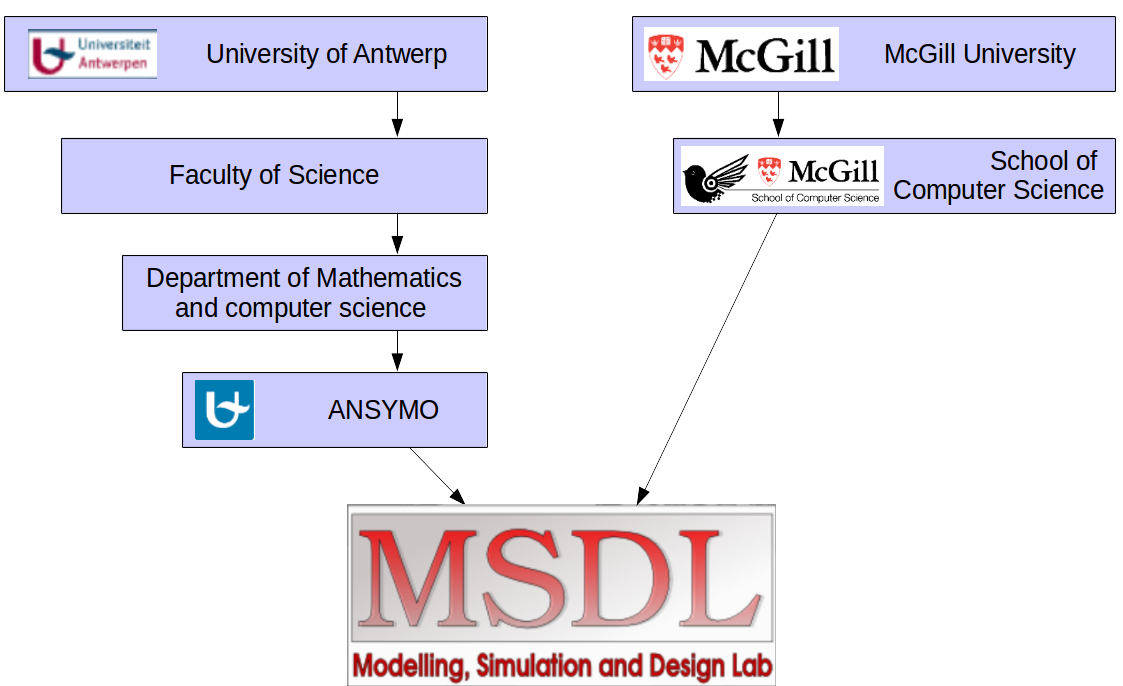
\includegraphics[width=0.8\linewidth]{msdl_organisation}

  \caption{Position of MSDL}
  \label{fig:msdl_org}
\end{figure}

The MSDL laboratory has members in two schools, most part of these members are in the University of Antwerp but there are some PhD students in the McGill University. McGill University is an English-language public research university in Montreal, Canada. You can see on the Figure \ref{fig:msdl_org} a description of the organization of these universities\footnote{Only departments which belongs msdl were presented.} and the position of MSDL in this organization.


\section{Description of MSDL}


\begin{figure}[!h]
  \centering
  
\includegraphics[width=0.6\textwidth]{MSDLbanner}
  \caption{MSDL banner}
  \label{fig:msdl}
\end{figure}


\begin{quotation}
<<The Modelling, Simulation and Design lab (MSDL) headed by Prof. Hans Vangheluwe is part of the School of Computer Science of McGill University in Montreal, Quebec, Canada and of the AnSyMo (Antwerp Systems and software Modelling) group in the department of Mathematics and Computer Science of the University of Antwerp, Antwerp, Belgium. The MSDL has projects, researchers and students in both locations.>>\cite{msdl}
\end{quotation}


So MSDL is a laboratory of Modelling. Modelling is an important field of computer science because it captures ideas in complex systems without all the accidental complexity of traditional software development. Models that have a well defined semantics also permit to create software without programming. I had the opportunity during my internship to participate in a presentation of all research subject. The Figure \ref{fig:subject} is a not exhaustive list of all research topics discussed in MSDL. The ones most related to my subject are \textit{Simulation} and \textit{Analysis, Validation, Verification, Testing, and Accreditation}.


\begin{figure}[h]
  \centering
  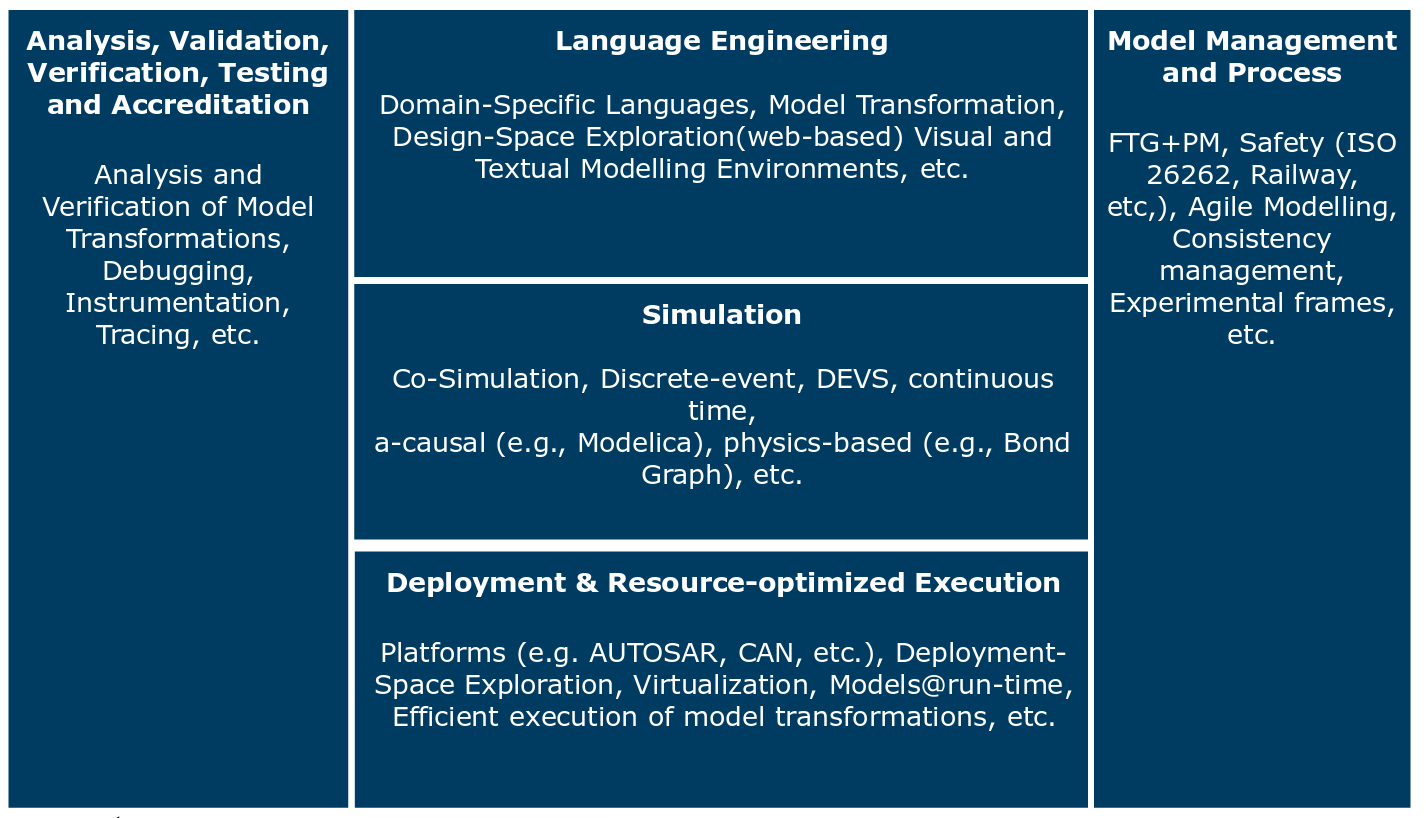
\includegraphics[width=\linewidth]{research}
  \caption{Research topics}
  \label{fig:subject}
\end{figure}



%%% Local Variables:
%%% mode: latex
%%% TeX-master: "../rapport_de_base"
%%% End:
